% !TeX document-id = {5986425d-2453-4c25-8285-071593d24d0f}
% !TeX TXS-program:compile = txs:///pdflatex/[--shell-escape]
\documentclass{article}

\usepackage[utf8]{inputenc}
\usepackage[T1]{fontenc}
\usepackage{color}
\usepackage{soul}
\usepackage{amsmath}
\usepackage{amssymb}
\usepackage{listings}
\usepackage{minted}
\usepackage{hyperref}
\usepackage{graphicx}
\usepackage{calc}
\usepackage{enumitem}
\usepackage{standalone}

\graphicspath{{img/}}
\setlength{\parindent}{0pt}

\begin{document}

\section{USRP Hardware Problems} 

\subsection{How It Is Supposed to Work}

The following plots show the output of a successful measurement with two USRPs using CSMA/CA, although measurement 4 is a little bit messed up as well. Note that wrong x-axis on the line chart has been fixed by the time writing this.

\bigskip

\textbf{Note:} Always take a look at the y-axis scaling. While such data representation might confuse the skimming reader it allows for higher resolution. Also note that not every plot adds more information, this also has the purpose of showcasing different plot types.

\begin{figure}[h] \label{usrp-success-1}
	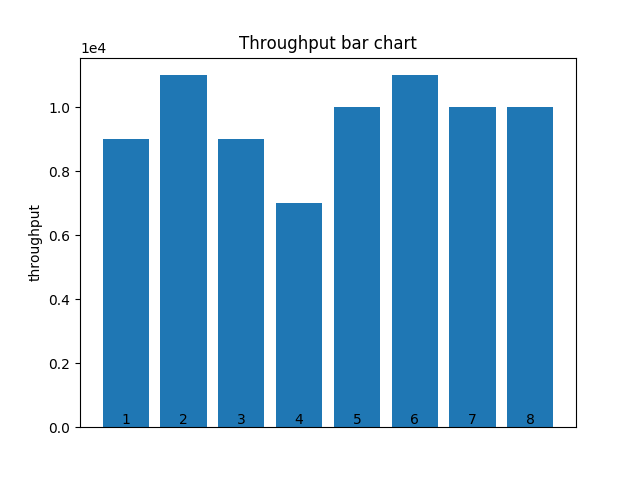
\includegraphics[width=\textwidth]{usrp_success_tp_bar}	
\end{figure}

\begin{figure}[ht] \label{usrp-success-2}
	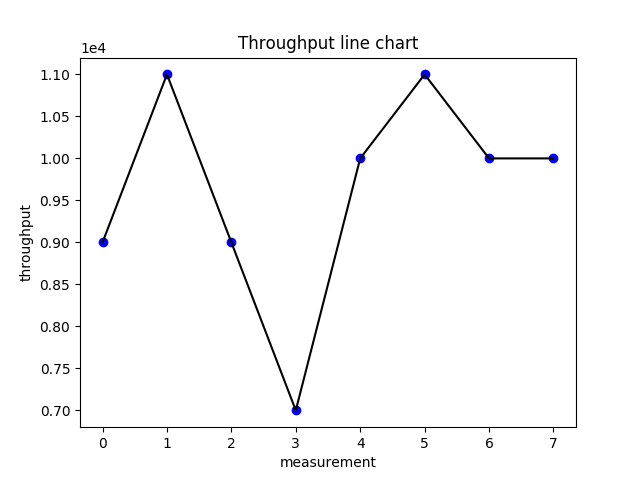
\includegraphics[width=\textwidth]{usrp_success_tp_line}	
\end{figure}

\begin{figure}[h] \label{usrp-success-3}
	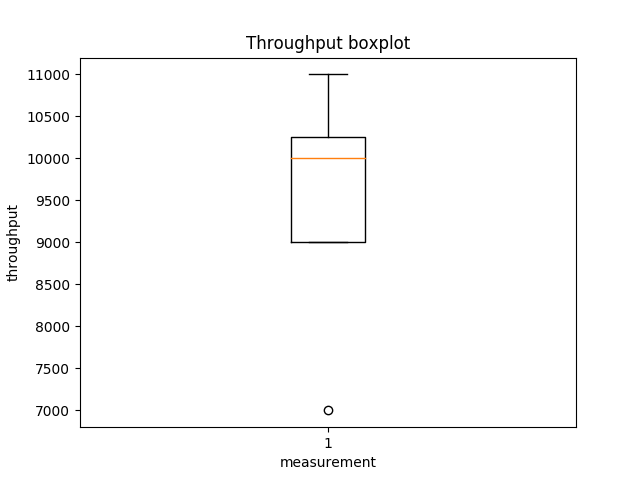
\includegraphics[width=\textwidth]{usrp_success_tp_boxplot}	
\end{figure}

\begin{figure}[h] \label{usrp-success-4}
	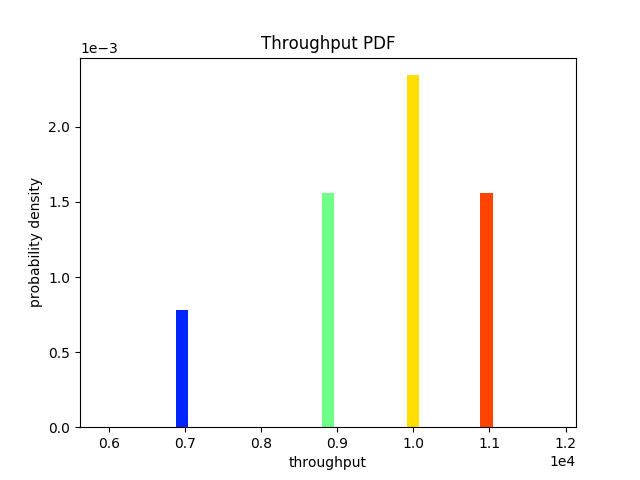
\includegraphics[width=\textwidth]{usrp_success_tp_pdf}	
\end{figure}

\begin{figure}[h] \label{usrp-success-5}
	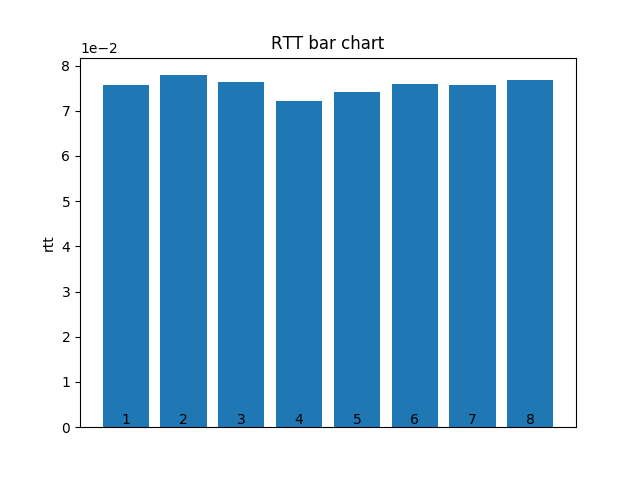
\includegraphics[width=\textwidth]{usrp_success_rtt_bar}	
\end{figure}

\begin{figure}[h] \label{usrp-success-6}
	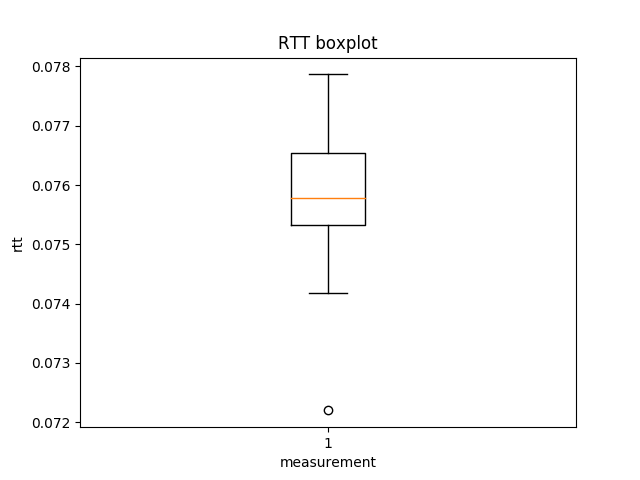
\includegraphics[width=\textwidth]{usrp_success_rtt_boxplot}	
\end{figure}

\begin{figure}[h] \label{usrp-success-7}
	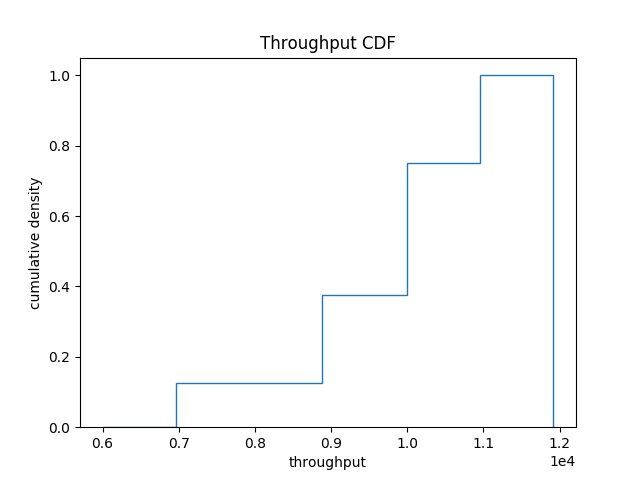
\includegraphics[width=\textwidth]{usrp_success_tp_cdf}	
\end{figure}

\clearpage

\subsection{Failure Pattern 1}

The following six figures visualize an issue I'm experiencing with the USRPs whose origin I have difficulties to track down. In seemingly random patterns the devices fail for the rest of the transmission. To make matters worse, it is not obvious whether the problem is hardware-related or software-related. Let me first explain what happens in the following plots, though.

\bigskip

In the throughput bar chart it is obvious the device failed during the measurements 2 and 20. The logs of the measurement and this suggest that this could very well be a software problem.
After 17 seconds the sender doesn't send any frames anymore (frame\_probe 850 is not reached anymore.) Once the sender fails it doesn't recover until the measurement script and the next measurement is launched, which is a reason to suspect a software failure on either my side or Gnu Radio's. 

\begin{figure}[h] \label{usrp-fails-4}
	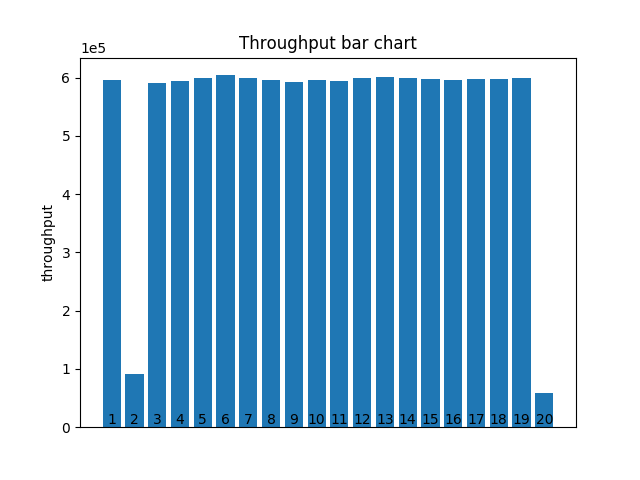
\includegraphics[width=\textwidth]{usrp_fail_tp_bar}	
\end{figure}

\begin{minted}[tabsize=4]{bash}
### This is from the measurements logs
Measurement 2/20 complete in 100 second(s).
# ... cut ...
Measurement 2/20 complete in 83 second(s).
++++ frame_probe ID: 860 receives a frame at time 71.8424s ++++
++++ frame_probe ID: 1010 receives a frame at time 71.846s ++++
++++ frame_probe ID: 890 receives a frame at time 71.8708s ++++
the 100th message counter  has been visited 89 times  
++++ frame_probe ID: 850 receives a frame at time 71.9534s ++++
INFO: Detected an invalid packet at item 8544
INFO: Parser returned #f
++++ frame_probe ID: 860 receives a frame at time 71.9941s ++++
++++ frame_probe ID: 1010 receives a frame at time 71.9994s ++++
++++ frame_probe ID: 890 receives a frame at time 72.0241s ++++
the 100th message counter  has been visited 90 times  
++++ frame_probe ID: 850 receives a frame at time 72.0925s ++++
INFO: Detected an invalid packet at item 8640
INFO: Parser returned #f
++++ frame_probe ID: 860 receives a frame at time 72.1332s ++++
++++ frame_probe ID: 1010 receives a frame at time 72.1437s ++++
++++ frame_probe ID: 890 receives a frame at time 72.1685s ++++
the 100th message counter  has been visited 91 times  
Measurement 2/20 complete in 82 second(s).
Measurement 2/20 complete in 81 second(s).
Measurement 2/20 complete in 80 second(s).
Measurement 2/20 complete in 79 second(s).
Measurement 2/20 complete in 78 second(s).
Measurement 2/20 complete in 77 second(s).
Measurement 2/20 complete in 76 second(s).
Measurement 2/20 complete in 75 second(s).
Measurement 2/20 complete in 74 second(s).
Measurement 2/20 complete in 73 second(s).
Measurement 2/20 complete in 72 second(s).
# ... cut ...
Measurement 2/20 complete in 2 second(s).
Measurement 2/20 complete in 1 second(s).
\end{minted}

\begin{figure}[h] \label{usrp-fails-5}
	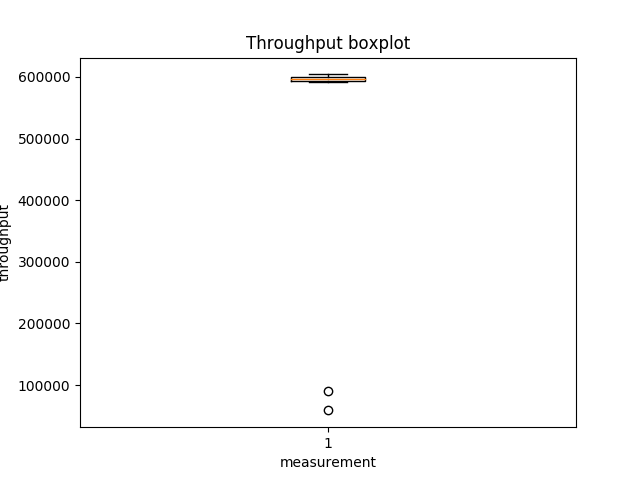
\includegraphics[width=\textwidth]{usrp_fail_tp_boxplot}
	
\end{figure}

\begin{figure}[h] \label{usrp-fails-6}
	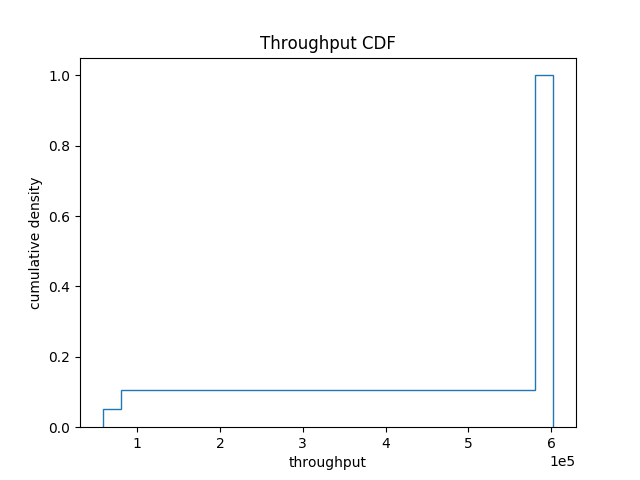
\includegraphics[width=\textwidth]{usrp_fail_tp_cdf}	
\end{figure} 

\begin{figure}[h] \label{usrp-fails-1}
	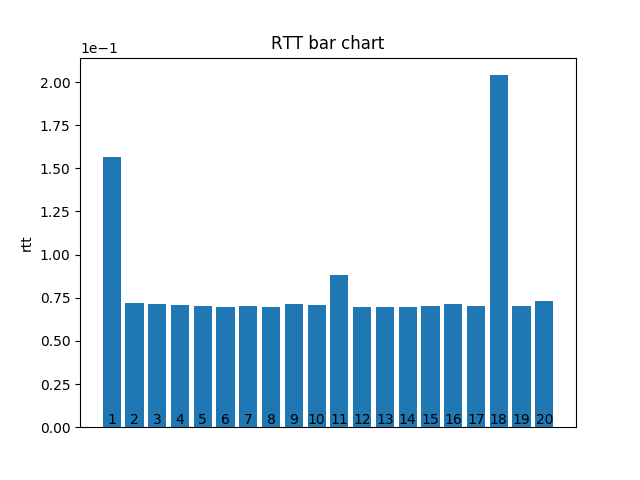
\includegraphics[width=\textwidth]{usrp_fail_rtt_bar}
	
\end{figure} 

\begin{figure}[h] \label{usrp-fails-2}
	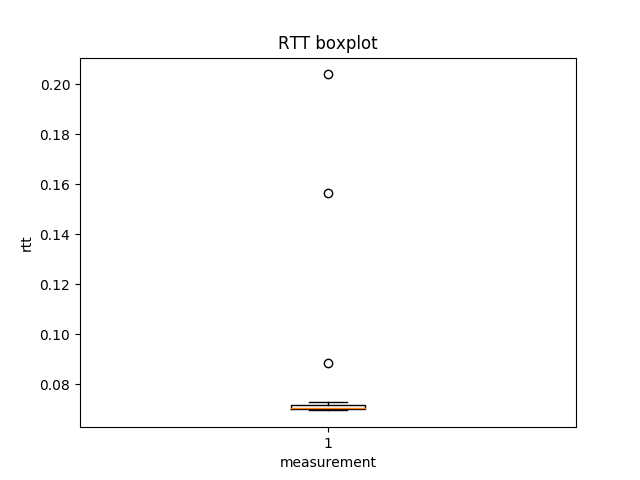
\includegraphics[width=\textwidth]{usrp_fail_rtt_boxplot}
\end{figure}

\begin{figure}[h] \label{usrp-fails-3}
	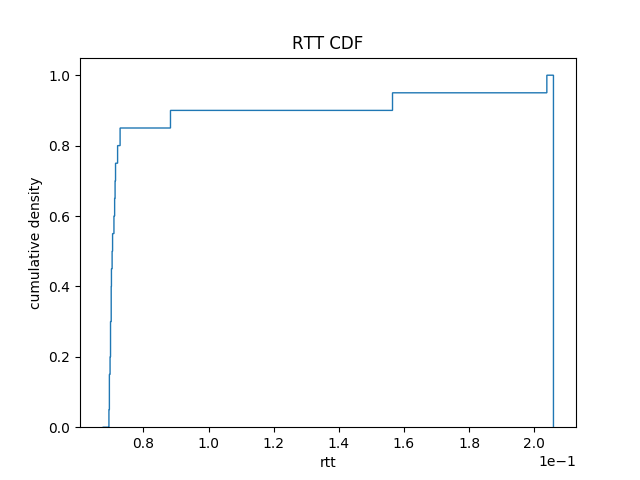
\includegraphics[width=\textwidth]{usrp_fail_rtt_cdf}
\end{figure}

\clearpage

\subsection{Failure Pattern 2}

\end{document}